\documentclass[tikz,border=10pt]{standalone}
\usetikzlibrary{arrows.meta}
\pagecolor{white}
\begin{document}
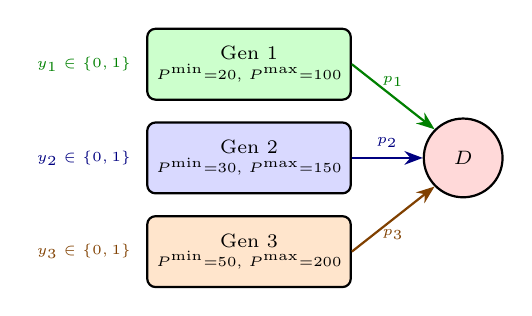
\begin{tikzpicture}[scale=0.85,
  gen/.style={draw, thick, rounded corners=3pt, minimum width=1.4cm,
              minimum height=0.9cm, font=\scriptsize, align=center},
]
  \node[gen, fill=green!20]  (g1) at (0, 2.2)  {Gen 1\\[-1pt]{\tiny $P^{\min}{=}20$, $P^{\max}{=}100$}};
  \node[gen, fill=blue!15]   (g2) at (0, 0.8)  {Gen 2\\[-1pt]{\tiny $P^{\min}{=}30$, $P^{\max}{=}150$}};
  \node[gen, fill=orange!20] (g3) at (0, -0.6) {Gen 3\\[-1pt]{\tiny $P^{\min}{=}50$, $P^{\max}{=}200$}};
  \node[draw, thick, circle, fill=red!15, minimum size=1cm,
        font=\scriptsize\bfseries] (d) at (3.2, 0.8) {$D$};
  \draw[-{Stealth}, thick, green!50!black] (g1.east) -- node[above, font=\tiny] {$p_1$} (d.north west);
  \draw[-{Stealth}, thick, blue!50!black]  (g2.east) -- node[above, font=\tiny] {$p_2$} (d.west);
  \draw[-{Stealth}, thick, orange!50!black](g3.east) -- node[below, font=\tiny] {$p_3$} (d.south west);
  \node[font=\tiny, green!50!black, anchor=east] at (g1.west) {$y_1 \in \{0,1\}$\;};
  \node[font=\tiny, blue!50!black, anchor=east]  at (g2.west) {$y_2 \in \{0,1\}$\;};
  \node[font=\tiny, orange!50!black, anchor=east]at (g3.west) {$y_3 \in \{0,1\}$\;};
\end{tikzpicture}
\end{document}
